
\documentclass[twoside,onecolumn]{article}

\usepackage{blindtext} % Package to generate dummy text throughout this template 

%\usepackage[sc]{mathpazo} % Use the Palatino font
\usepackage[T1]{fontenc} % Use 8-bit encoding that has 256 glyphs
\linespread{1.05} % Line spacing - Palatino needs more space between lines
\usepackage{microtype} % Slightly tweak font spacing for aesthetics
\usepackage{float}
\usepackage{hyperref}
 \usepackage{amsmath}
 \usepackage{booktabs}
 \usepackage{amssymb}
 \usepackage{amsthm}
 \usepackage{tabularx} %tabelle
 \usepackage{tikz} %circuiti
 \usepackage{enumerate}
 \usepackage{pgfplots}
 \usepackage{subcaption}
\usepackage[toc,page]{appendix}
 \usepackage[export]{adjustbox}
 \usepackage{caption}
 \usepackage{subfig}
 \usepackage{sidecap}
 \usepackage{algorithm}

 \usepackage{graphicx}
 \theoremstyle{definition}
  \usepackage{multicol}
  \usetikzlibrary{arrows}
  \usepackage{algpseudocode}
\usepackage{multirow}
\usepackage{mathtools}
\usepackage{array, caption}
\usepackage{graphicx}
\usepackage{makecell}
  \usepackage{xparse}

\NewDocumentCommand{\codeword}{v}{%
\texttt{\textcolor{black}{#1}}%
}

\usepackage[english]{babel} % Language hyphenation and typographical rules

\usepackage[hmarginratio=1:1,top=32mm,columnsep=20pt]{geometry} % Document margins
\usepackage[hang, small,labelfont=bf,up,textfont=it,up]{caption} % Custom captions under/above floats in tables or figures
\usepackage{booktabs} % Horizontal rules in tables

\usepackage{lettrine} % The lettrine is the first enlarged letter at the beginning of the text

\usepackage{enumitem} % Customized lists
\setlist[itemize]{noitemsep} % Make itemize lists more compact

\usepackage{titlesec} % Allows customization of titles
\titleformat{\section}[block]{\large\scshape\centering}{\thesection.}{1em}{} % Change the look of the section titles
\titleformat{\subsection}[block]{\large}{\thesubsection.}{1em}{} % Change the look of the section titles

\usepackage{hyperref} % For hyperlinks in the PDF

\title{Lab 3: Edge, lines and circles detection } % Article title
\author{Nicole Zattarin}
\date{} 
\begin{document}

% Print the title
\maketitle

\begin{abstract}
ciao belli
\end{abstract}
\section{Setup and parameters tuning}


At \href{https://github.com/nicolezattarin/Computer-Vision/tree/main/edge_detection}{this link} we provide a possible implementation of a program that, given an image, performs edge, lines and circles detection. The executable is structured in order to receive from command line a path to an image, a path to a file of parameters and three boolean variables, that allow the user to decide if he wants to tune the parameters by means of trackbars, i.e. :
\begin{verbatim}
 ./main <image path> <params file path> <tune canny> <tune HoughLines> <tune HoughCircles>
\end{verbatim}
For instance, the following example launch the program in order to process the image \codeword{road2.png} getting initial parameters from the file \codeword{paramsRoad2.txt} and perform only the tuning of Canny parameters:
\begin{verbatim}
 ./main images/road2.png params/paramsRoad2.txt 1 0 0 
\end{verbatim}
Note that once a tuner flag is set to 1, the code runs up to that tuning phase with the parameters provided in the file, then once the tuning window is closed, the execution stops as well.
The idea is that we can get a good result by tuning a detector at a time, i.e. tune a detector for each run of the code, moreover, everything is made pretty efficient by the usage of trackbars. Therefore, first we tune Canny, see an example of interface in Figure \ref{fig:tuningedge}, and we write down the best set of parameters in the \codeword{.txt} file. Then, in two successive runs, we do the same with HoughLines, see Figure \ref{fig:tuningline}, and HoughCircles. Trackbars are useful to see in real time how the output of a detector is affected by parameters change, for instance in Figure \ref{fig:tuningline} we can observe lines appearing and disappearing according to the angle range and to the threshold. At the end of this tuning process the chosen parameters are printed on the screen, so that we can register them manually in the \codeword{.txt} file, in such a way that running the algorithm on the same image will return the desired result and save the corresponding images in a specific folder. To summarize, the workflow should look like:
\begin{verbatim}
./main images/road2.png params/paramsRoad2.txt 1 0 0 // manually tune params, update params file
./main images/road2.png params/paramsRoad2.txt 0 1 0 // manually tune  params, update params file
./main images/road2.png params/paramsRoad2.txt 0 0 1 // manually tune params, update params file
./main images/road2.png params/paramsRoad2.txt 0 0 0 // get all final results!
\end{verbatim}

Trackbars callbacks are collected in \codeword{trackbars.h}, while \codeword{utils.h} contains all the functions that can be useful to manipulate images, lines, circles and draw on the image itself.
Finally, note that each of the image requires a specific tuning and a specific processing in order to get the final result, this is performed with functions provided in \codeword{images_processing.h}. Therefore, running the code on a generic image won't give back the same result as on the samples ones, unless one creates a specific function to deal with it.

\begin{figure} \centering
\begin{subfigure}{0.5\textwidth}
  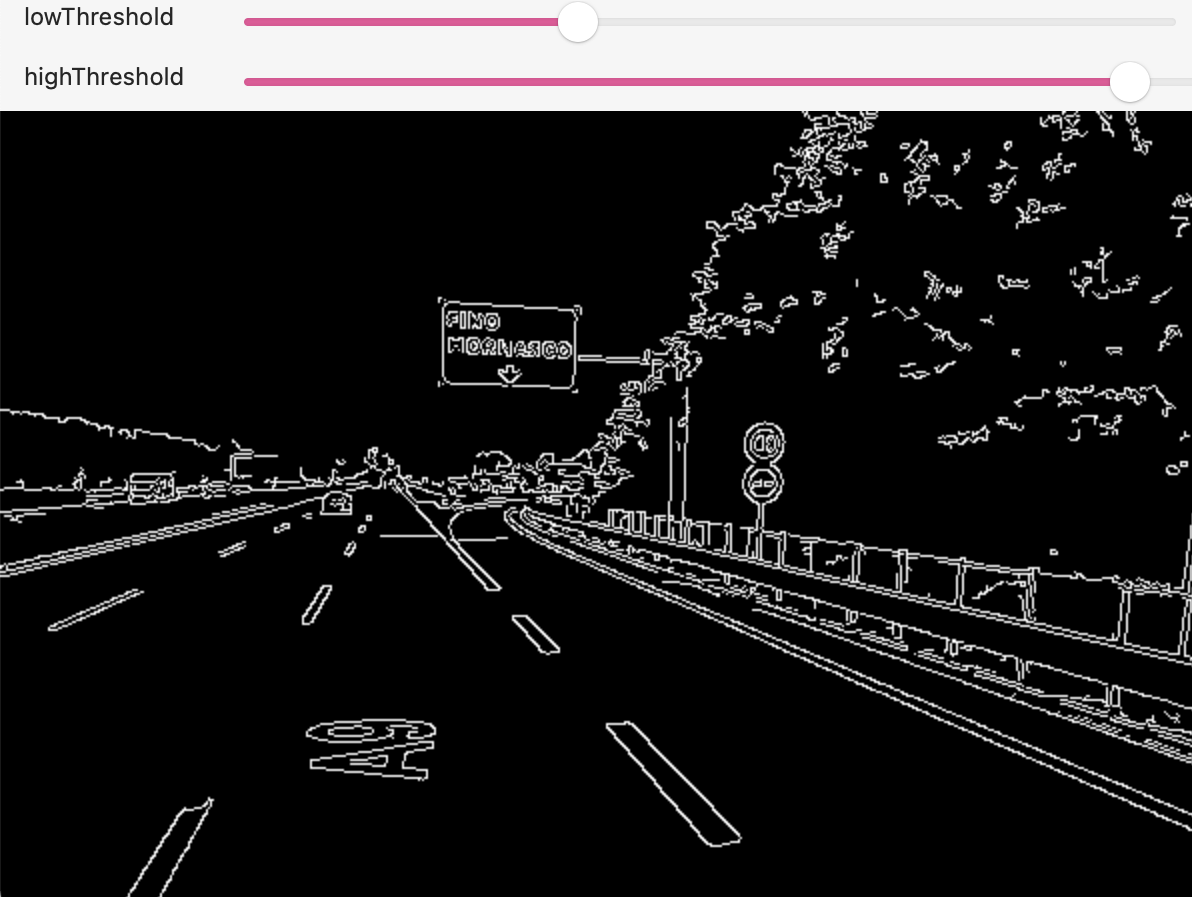
\includegraphics[width=\textwidth]{../results/tuningEdge.png}
\caption{ Example of interface for Canny parameters tuning, i.e. lower and higher thresholds.}\label{fig:tuningedge}
\end{subfigure} \quad
\begin{subfigure}{0.46\textwidth}
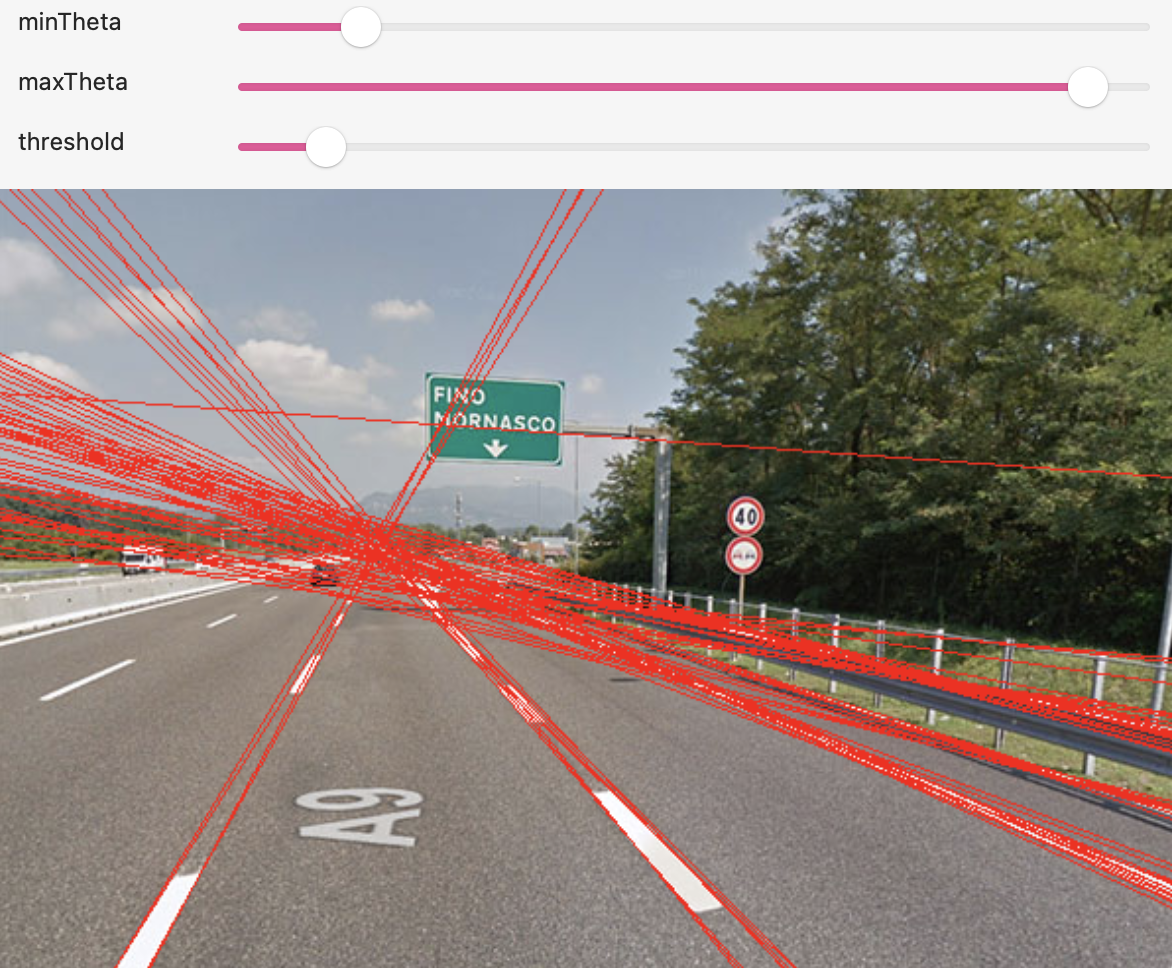
\includegraphics[width=\textwidth]{../results/tuningLines.png}
\caption{Example of interface for HoughLines parameters tuning, i.e. threshold and angle range.}\label{fig:tuningline}
\end{subfigure}\caption{Example of interface for a run in which we ask to tune the Canny parameters (a) and the HoughLines (b). Note that parameters are set randomly in this example, just to show that the image changes according to values inserted through the trackbar. }\label{fig:tuning}
\end{figure}


\section{Results}
We test edges, lines and circles detection of three images provided in the folder \codeword{images}, in particular \codeword{road2.png},  \codeword{road3.jpg} and \codeword{road4.jpg}.
The initial part of the processing is the same for all the images and consists of the following steps:
\begin{enumerate}
\item Load image and parameters, show the original image;
\item Apply Canny to the greyscale image, tune the parameters if it's the case and save the edge map;
\item Use the output of Canny, i.e. the edge map, to individuate lines within the image by means of HoughLines, tune the parameters in order to individuate only the boundaries of the street or of the street lane. Moreover, once the parameters are fixed, we fill the polygon determined by the lower points of two intersecting lines and the intersection point;
\item  Apply HoughCircles the greyscale image to the greyscale image to individuate circles, with particular attention to the most relevant parameters in order to detect only round street signs. Finally we fill them with the same color.
\end{enumerate}

In particular parameters to process image \codeword{road2.png} are shown in Table \ref{tab:r2}, while in Figure \ref{fig:road2} we provide three different steps of the image manipulation: original image in Figure \ref{fig:r2fig}, edge map in Figure \ref{fig:r2edges} and the final result in \ref{fig:r2circles}. Note that in the final result we show only the relevant lines and we fill in between only up to the intersection point. 

\begin{table}\centering
\begin{tabular}[t]{ |c|c|c| }
\hline
\multirow{8}{*}[6.5ex]{\rotatebox{90}{Canny}} 
 & apertureSize & 3 \\
 & threshold1  & 350 \\
 & threshold2 & 850\\  \hline
\end{tabular}
\hskip
\begin{tabular}[t]{ |c|c|c| }
\hline
\multirow{8}{*}[4ex]{\rotatebox{90}{HoughLines}} 
& rho &  1 \\
 & theta & 0.05 \\
 &threshold& 130\\
  & min theta  & 0\\ 
 & max theta  & CV PI\\ \hline
\end{tabular}
\hskip
\begin{tabular}[t]{ |c|c|c| }
\hline
\multirow{8}{*}[3ex]{\rotatebox{90}{HoughCircles}} 
& dp & 1 \\
& minDist & 1\\
& param1& 100 \\
& param2& 25 \\ 
& minRadius& 0 \\ 
& maxRadius & 10 \\ \hline
\end{tabular}
\caption{Parameters set for road2.png image, for all the three algorithms. } \label{tab:r2}
\end{table}


\begin{figure} \centering
\begin{subfigure}{0.8\textwidth}
  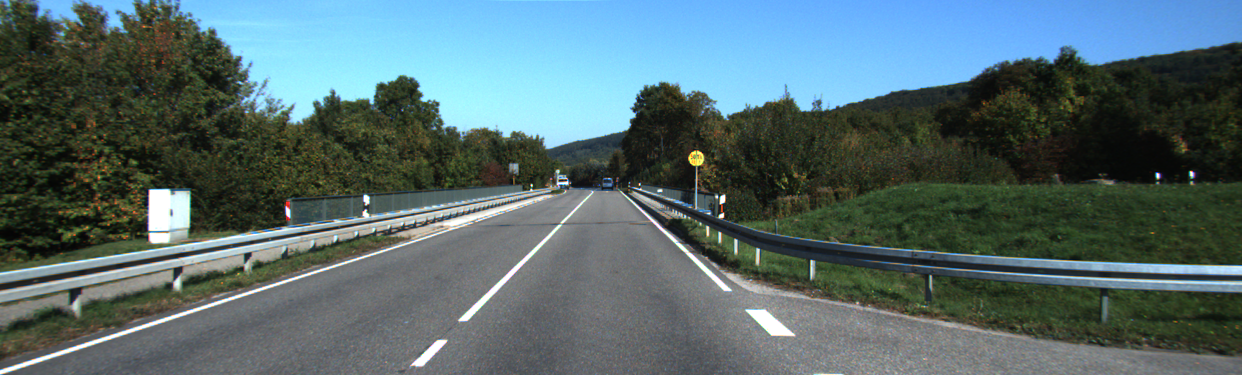
\includegraphics[width=\textwidth]{../images/road2.png}
\caption{Original image }\label{fig:r2fig}
\end{subfigure} \\
\begin{subfigure}{0.8\textwidth}
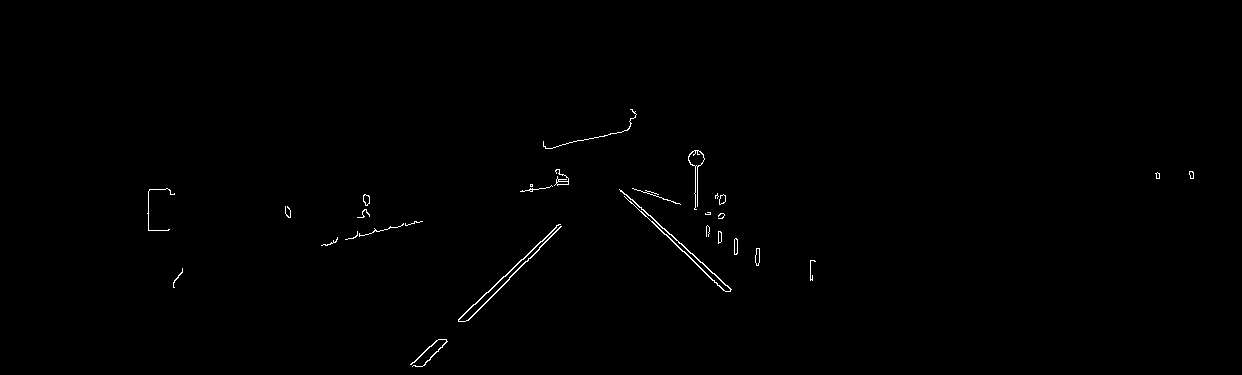
\includegraphics[width=\textwidth]{../results/edgeMap_road2.png}
\caption{Edge map after applying Canny to the greyscale image}\label{fig:r2edges}
\end{subfigure}
  \begin{subfigure}{0.8\textwidth}
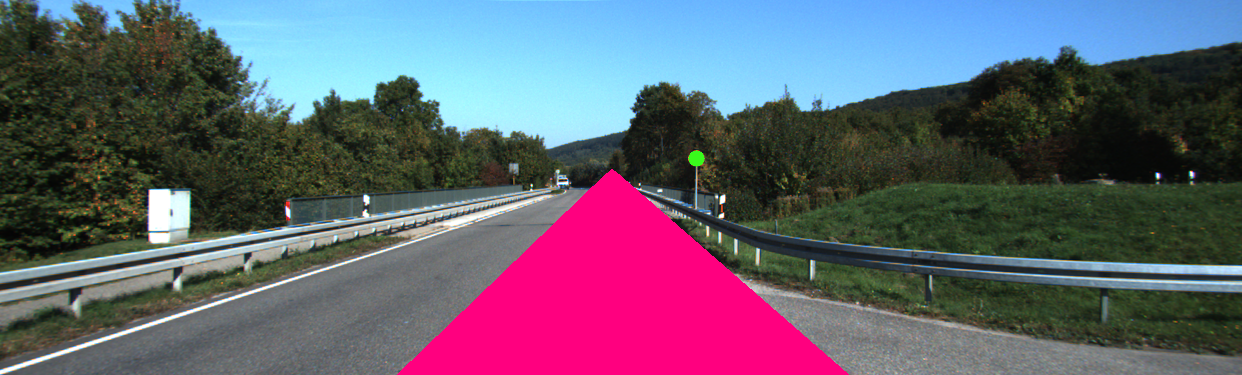
\includegraphics[width=\textwidth]{../results/Circles_road2.png}
\caption{Final result: circle street signs are filled in green, while the area between the intersected lines is filled in magenta}\label{fig:r2circles}
\end{subfigure}\caption{Three different steps of the image manipulation: original image in Figure \ref{fig:r2fig}, edge map in Figure \ref{fig:r2edges} and the final result in \ref{fig:r2circles}. }\label{fig:road2}
\end{figure}
For what concerns image \codeword{road3.jpg}, parameters are shown in Table \ref{tab:r3}, while images in Figure \ref{fig:road3}.

%ROAD3
\begin{table}\centering
  \begin{tabular}[t]{ |c|c|c| }
  \hline
  \multirow{8}{*}[6.5ex]{\rotatebox{90}{Canny}} 
   & apertureSize & 3 \\
   & threshold1  & 270 \\
   & threshold2 & 400\\  \hline
  \end{tabular}
  \hskip
  \begin{tabular}[t]{ |c|c|c| }
  \hline
  \multirow{8}{*}[4ex]{\rotatebox{90}{HoughLines}} 
  & rho &  1 \\
   & theta & 0.05 \\
   &threshold& 160\\
    & min theta  & 0\\ 
   & max theta  & 3\\ \hline
  \end{tabular}
  \hskip
  \begin{tabular}[t]{ |c|c|c| }
  \hline
  \multirow{8}{*}[3ex]{\rotatebox{90}{HoughCircles}} 
  & dp & 1 \\
   & minDist & 1\\
   & param1& 353 \\
    & param2& 31 \\ 
      & minRadius& 0 \\ 
   & maxRadius & 32 \\ \hline
  \end{tabular}
  \caption{Parameters set for road3.jpg image, for all the three algorithms.} \label{tab:r2}
  \end{table}

  
\begin{figure} \centering
\begin{subfigure}{0.45\textwidth}
  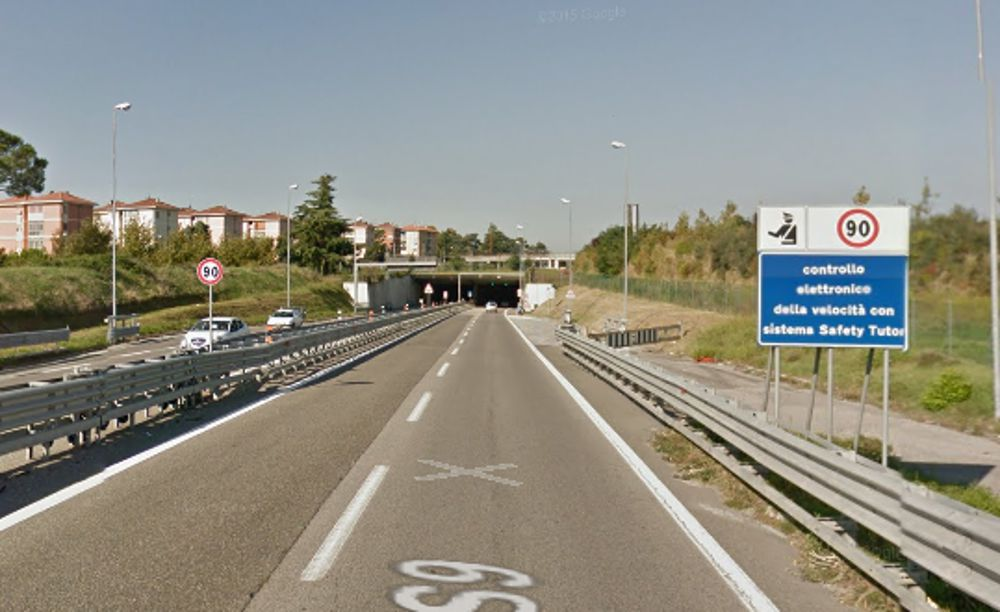
\includegraphics[width=\textwidth]{../images/road3.jpg}
\caption{ Original image}\label{fig:r3fig}
\end{subfigure} \quad
\begin{subfigure}{0.45\textwidth}
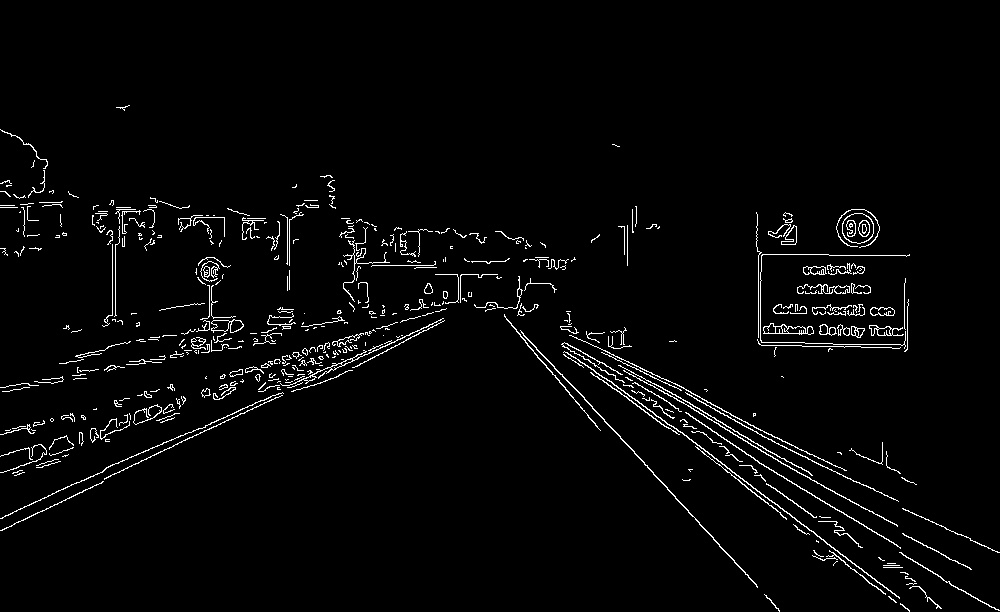
\includegraphics[width=\textwidth]{../results/edgeMap_road3.jpg}
\caption{Edge map after applying Canny to the greyscale image}\label{fig:r3edges}
\end{subfigure}\\
  \begin{subfigure}{0.6\textwidth}
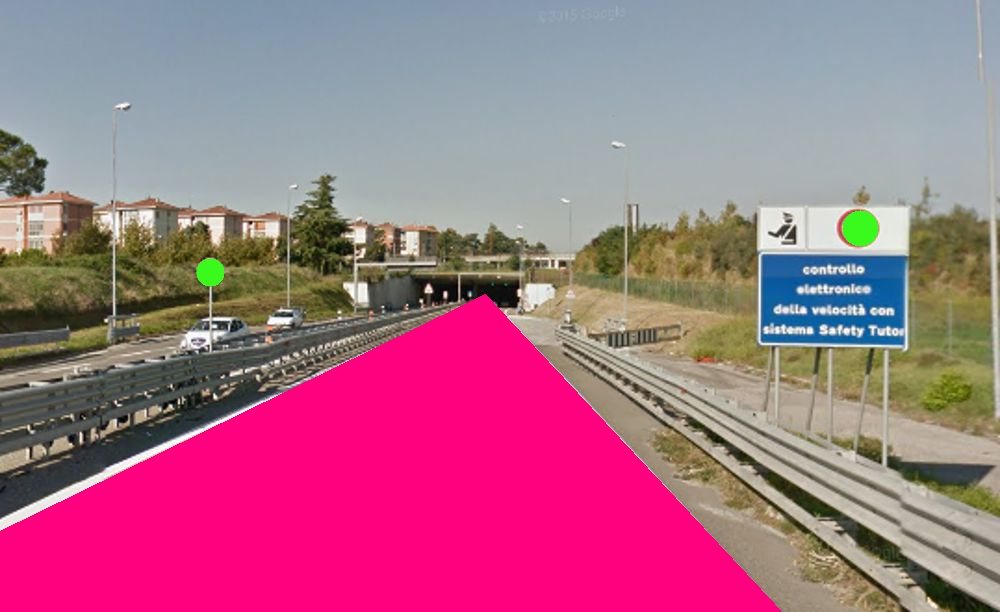
\includegraphics[width=\textwidth]{../results/Circles_road3.jpg}
\caption{Final result: circle street signs are filled in green, while the area between the intersected lines is filled in magenta }\label{fig:r3circles}
\end{subfigure}\caption{Three different steps of the image manipulation: original image in Figure \ref{fig:r3fig}, edge map in Figure \ref{fig:r3edges} and the final result in \ref{fig:r3circles}.}\label{fig:road3}
\end{figure}


%ROAD4
\begin{table}\centering
  \begin{tabular}[t]{ |c|c|c| }
  \hline
  \multirow{8}{*}[6.5ex]{\rotatebox{90}{Canny}} 
   & apertureSize & 3 \\
   & threshold1  & 450 \\
   & threshold2 & 730\\  \hline
  \end{tabular}
  \hskip
  \begin{tabular}[t]{ |c|c|c| }
  \hline
  \multirow{8}{*}[4ex]{\rotatebox{90}{HoughLines}} 
  & rho &  1 \\
   & theta & 0.05 \\
   &threshold& 62\\
    & min theta  & 1\\ 
   & max theta  & 3\\ \hline
  \end{tabular}
  \hskip
  \begin{tabular}[t]{ |c|c|c| }
  \hline
  \multirow{8}{*}[3ex]{\rotatebox{90}{HoughCircles}} 
  & dp & 1 \\
   & minDist & 1\\
   & param1& 67 \\
    & param2& 31 \\ 
      & minRadius& 0 \\ 
   & maxRadius & 14 \\ \hline
  \end{tabular}
  \caption{Parameters set for road4.jpg image, for all the three algorithms.} \label{tab:r2}
  \end{table}


\begin{figure} \centering
\begin{subfigure}{0.45\textwidth}
  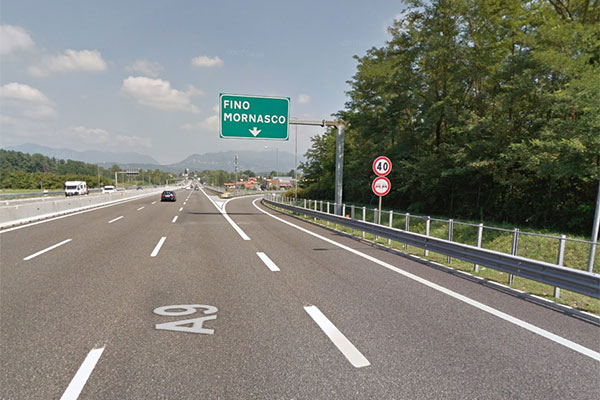
\includegraphics[width=\textwidth]{../images/road4.jpg}
\caption{Original image }\label{fig:r4fig}
\end{subfigure} \quad
\begin{subfigure}{0.45\textwidth}
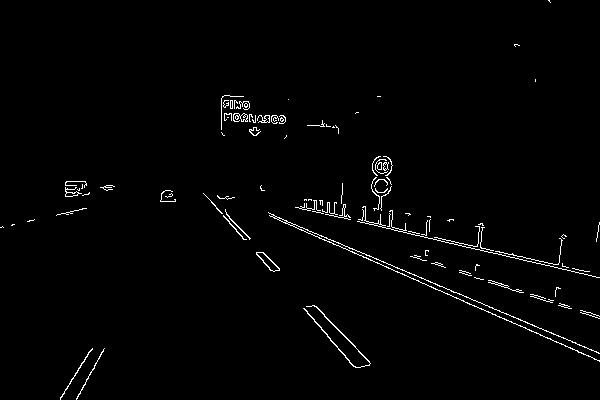
\includegraphics[width=\textwidth]{../results/edgeMap_road4.jpg}
\caption{Edge map after applying Canny to the greyscale image}\label{fig:r4edges}
\end{subfigure}\\
  \begin{subfigure}{0.6\textwidth}
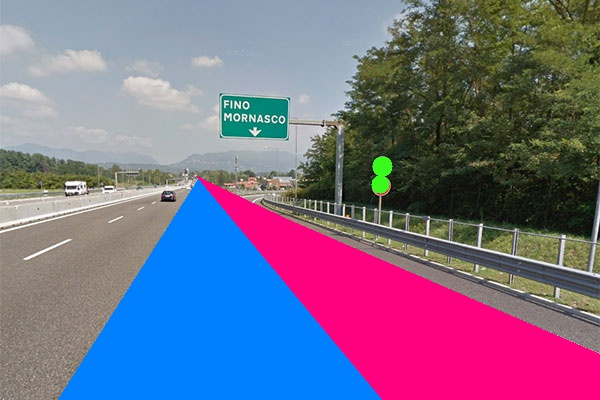
\includegraphics[width=\textwidth]{../results/Circles_road4.jpg}
\caption{Final result: circle street signs are filled in green, while the area between the intersected lines is filled in magenta and blue. Note that in this case we fill differently the two different areas in order to highlight the line in the middle.}\label{fig:r4circles}
\end{subfigure}\caption{Three different steps of the image manipulation: original image in Figure \ref{fig:r4fig}, edge map in Figure \ref{fig:r4edges} and the final result in \ref{fig:r4circles}. }\label{fig:road4}
\end{figure}



\end{document}

